\chapter{前言}
\renewcommand{\baselinestretch}{10.0} %設定行距
\pagenumbering{arabic} %設定頁號阿拉伯數字
\setcounter{page}{1}  %設定頁數
\fontsize{14pt}{2.5pt}\sectionef
\section{專案概述與目標}
本課程專案目標是開發一款能 web-based CoppeliaSim 場景中雙方或多方玩的遊戲產品,需要有場景與多輪車零組件設計(可使用各種 CAD 系統建立, 但必須提供完整的檔案下載連結)、控制程式、開會紀錄與逐字稿、各組員任務分配與執行過程影片及分組報告 pdf 檔案,最後在 w16 現場發表八人協同四週後所完成的產品,在 w17 各組採 OBS + Teams 以影片發表所完成的協同產品。
\begin{figure}[hbt!]
\begin{center}
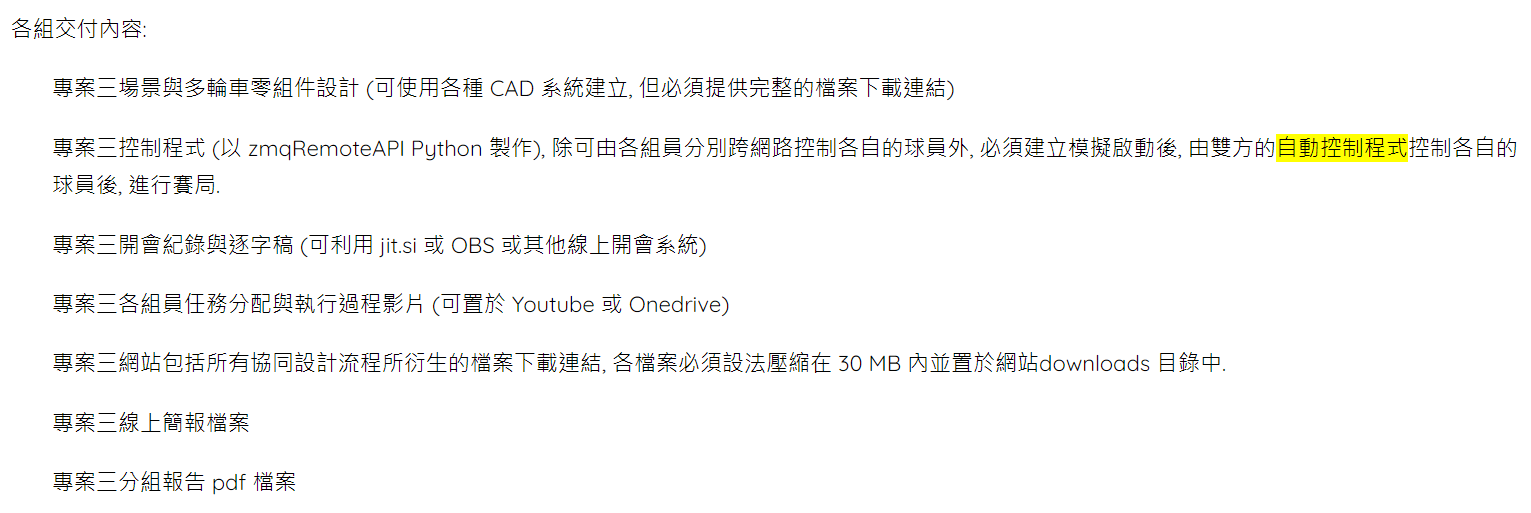
\includegraphics[height=10cm]{work}
\caption{\Large 專案目標}\label{專案目標}
\end{center}
\end{figure} 
\section{規則}
本專題設計理想為一款足球遊戲,比賽一開始球會置於場中央,遊戲開始後雙方即
可鍵盤操控機器人,透過防隊友間的傳球並將球送至球門即可得分。\\
遊戲規則如下:\\
\begin{enumerate}
\item 球送至敵方球門即得一分。\\
\item 時間內進球數多的一方獲勝。\\
\item 球進入球框後會回到原位。\\
\item 球出界後會回到原位。\\
\end{enumerate}
\renewcommand{\baselinestretch}{0.5} %設定行距